%
%     hw7_bbordwell.tex
%     Baylee Bordwell (baylee.bordwell@colorado.edu)
%     Based on the template by Benjamin Brown (bpbrown@colorado.edu)
%     Aug 27, 2014
%
%     Problem set 7 for ASTR/ATOC 5540, Mathematical Methods, taught at
%     University of Colorado, Boulder, Fall 2014.
%
%

\documentclass[10pt, preprint]{aastex}
% formatting based on 2014 NASA ATP proposal with Jeff Oishi

%%%%%%begin preamble
\usepackage[hmargin=1in, vmargin=1in]{geometry} % Margins
\usepackage{hyperref}
\usepackage{url}
\usepackage{times}
\usepackage{natbib}
\usepackage{graphicx}
\usepackage{amsmath}
\usepackage{amsfonts}
\usepackage{amssymb}
\usepackage{pdfpages}
\usepackage{import}
% for code import
\usepackage{listings}
\usepackage{color}
\usepackage{ragged2e}

\hypersetup{
     colorlinks   = true,
     citecolor     = gray,
     urlcolor       = blue
}

%% headers
\usepackage{fancyhdr}
\pagestyle{fancy}
\lhead{ASTR/ATOC 5540}
\chead{}
\rhead{name: Baylee Bordwell}
\lfoot{Problem Set 7}
\cfoot{\thepage}
\rfoot{Fall 2014}
% no hline under header
\renewcommand{\headrulewidth}{0pt}

\newcommand{\sol}{\ensuremath{\odot}}

% make lists compact
\usepackage{enumitem}
%\setlist{nosep}

%%%%%%end preamble


\begin{document}
\section*{Problem Set 7: Analyzing Kepler Data}
\begin{enumerate}
\item I detrended the Kepler data with an $N=3$ polynomial using the QR solution written in previous weeks' assignments. To check the fidelity of my detrended solution with that of Kepler, I looked at the L2 norm, which yielded a value of 2.20. Figure \ref{fig1} shows the two detrended solutions and their residual for visual confirmation of their agreement.
\begin{figure}[!ht]
\centering
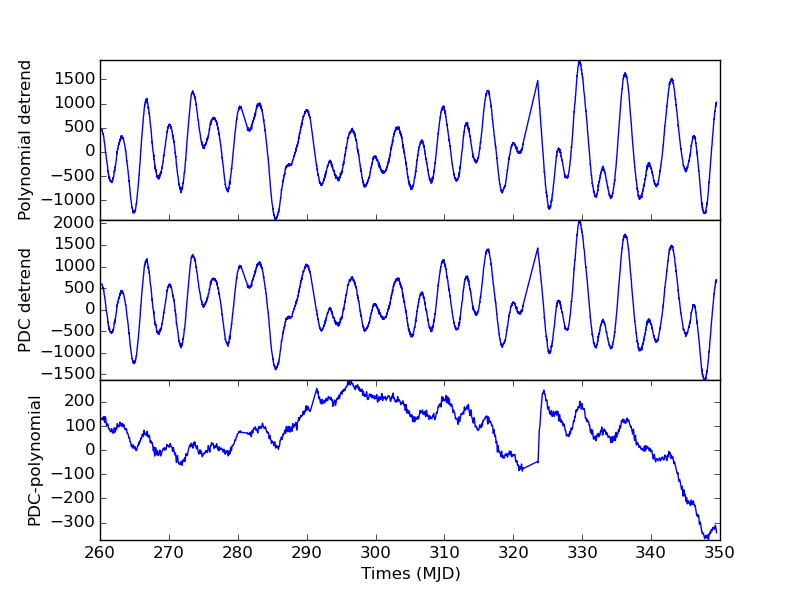
\includegraphics[width=3in]{hw7_fig1.png}
\caption{\centering \label{fig1}}
\end{figure}


\item And they match!
\begin{figure}[!ht]
\centering
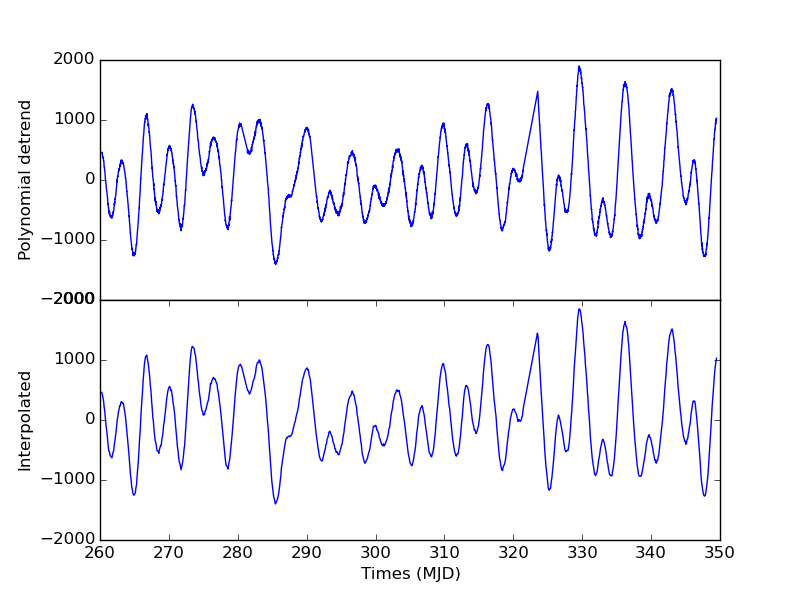
\includegraphics[width=3in]{hw7_fig2.png}
\caption{\centering \label{fig2}}
\end{figure}

\item The \verb|np.fft.fft()| function returns the coefficients first running from the zero frequency value to the highest frequency, which abutts the largest negative frequency and continue back up to the zero frequency. The frequency corresponding in FFT[0] is the zero frequency component of the data, and the coefficient typically shows you how much aperiodic noise is present in your data. The function took .324 ms to transform the interpolated data set.

\item Figure \ref{fig3} shows the power spectrum over the positive frequencies based on our $N=3$ detrended polynomial. I chose to plot with just the y-axis on a log scale, as having the x-axis on a log scale didn't really highlight any specific characteristics of the data.
\begin{figure}[!ht]
\centering
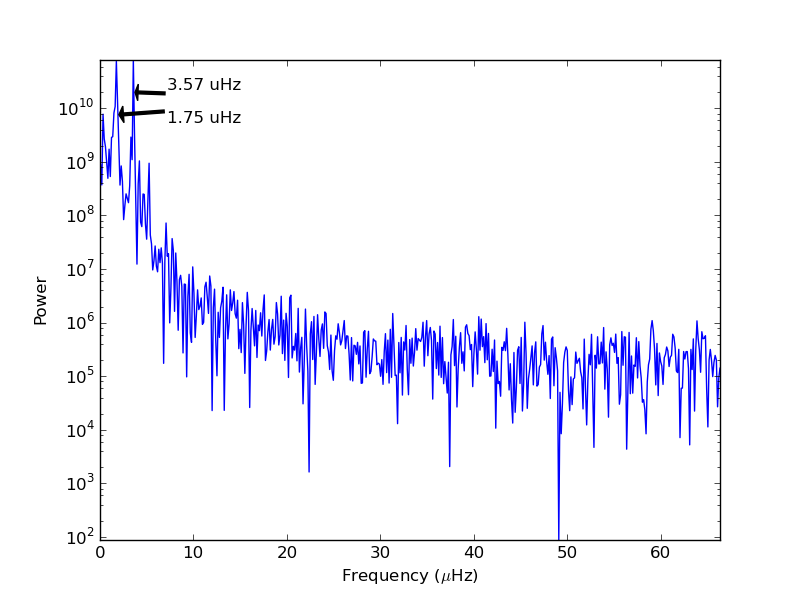
\includegraphics[width=3in]{hw7_fig3.png}
\caption{\centering \label{fig3}}
\end{figure}
 
\item Figure \ref{fig3} shows the two highest peaks in the power spectrum, located at 1.7507 and 3.5662 $\mu$Hz, or at periods of 6.6111 and 3.2455 days. Periods on this scale might represent the resonance of a fundamental frequency and second overtone in a double mode or bump cepheid variable star.\footnote{Kawaler, S.D. ``\emph{Learning physics from the stars: It's all in the coefficients.}'' Asteroseismology. Cambridge University Press. 2014. 32-59.} In general, these bumps likely reflect the effect of some stellar pulsation, or even a possible rotational effect.


\item Based on examination of Figure \ref{fig4}, the assumption that the data is periodic is a good one. When examining the points where copies of the time series were stitched together (highlighted in red in Figure \ref{fig4}, the alignment of the data appears very good. Detrending the data has helped by forcing the data to generally oscillate vertically around one horizontal line, allowing alignment of the data at the head and tail. Even after detrending, however, the data is not quite oscillating evenly about 0, due to the complex structure of different periods constibuting to its structure. If two points ten days behind and ahead of the original times series are considered (see green lines in Figure \ref{fig4}, then this trend is obvious. There are also probably discontinuities in the first derivative where the data sets are connected.
\begin{figure}[!ht]
\centering
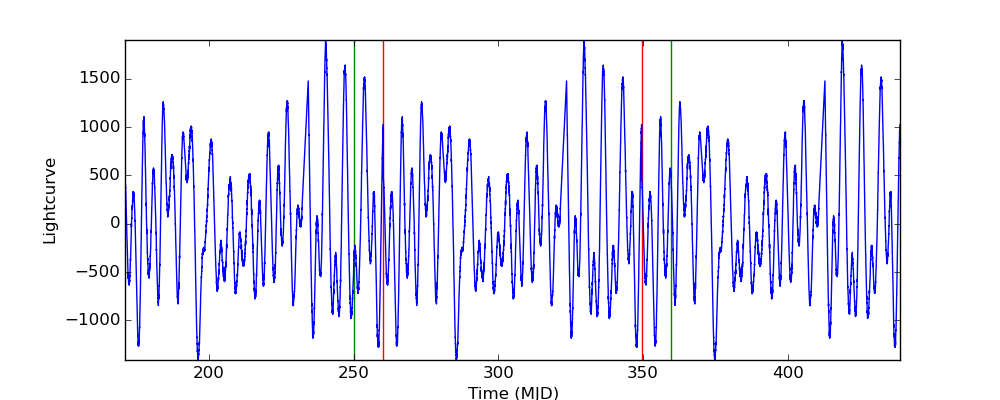
\includegraphics[width=6in]{hw7_fig4.png}
\caption{\centering \label{fig4}}
\end{figure}


\end{enumerate}

Code used in this assignment can be found at \url{https://github.com/brbordwell/ASTR_5540/HW7}
\end{document}
